\section{The MCP Inspector and its published vulnerability}
\label{sec:inspector}

The previous section established which parts of an MCP tool definition have an enforcer and which
rest on trust, and that no deadline travels with a request (\cref{sec:mcpcontract}). This section
examines these findings through the MCP Inspector, the tool that developers use to test MCP
servers, and asks what such a test can and cannot show. The question matters because the Inspector
receives exactly what any host receives, so its limits are the limits of every host. We then study
a published vulnerability in the Inspector itself, which shows that a component that starts
processes on request must check who sends the request.

\subsection{A host with no model}
\label{sec:inspector-host}

The \textbf{MCP Inspector} is the MCP project's reference tool for testing and debugging MCP
servers, and in MCP's terms it is a host with no model \citep{mcp-inspector}. A developer connects
it to a server, reads the server's tool definitions and calls its tools by hand. The same package
also offers a command-line mode and a terminal mode, which work without a browser.

The Inspector consists of a web client and a proxy. The \textbf{web client} is a page in the
developer's browser, on which the developer reads tool definitions, fills in arguments and reads
results. The \textbf{proxy} is the Inspector's local program on the developer's machine, and it
holds every connection to the servers. It also starts, as a subprocess, each server that uses the
stdio transport (\cref{sec:mcp-server}).

The web client sends its requests to the proxy, and the proxy forwards them to the server. A page
in a browser cannot start a process on its machine, so the proxy does this on the page's behalf.

In current versions, the proxy accepts connections only from the developer's own machine. When it
starts, it generates a \textbf{session token}, a secret that the proxy requires on every request to
its API. Version 0.14.1 added these protections to close the vulnerability described in
\cref{sec:inspector-cve}.

As a host (\cref{sec:mcp}), the Inspector creates one client for each server it connects to, and
that client sends the same \demoref{tools/list} and \demoref{tools/call} requests as the client of
any other host. The Inspector differs from other hosts in that its user works in a browser and it
has no model. A person chooses each call and types its arguments, where another host would pass on
the model's tool call.

The Inspector displays the full tool list that a host receives, with every field of each tool
definition. This is more than a model sees, because a host passes the model only the name, the
description and the input schema of each tool (\cref{sec:mcp-native}).

Because the messages are the same, testing a server in the Inspector shows exactly what the server
sends to any host. Since no model takes part, each result reflects the server alone.

\subsection{Errors and timeouts in the Inspector}
\label{sec:inspector-errors}

Connected to a real server, the Inspector makes several properties of MCP directly visible. The
server here is the edit server of \cref{sec:mcp}, which serves the \demoref{edit} tool of our
running agent, \msa{}, from a separate process. Calls to it show the following:
\bi
\item \textbf{A successful call.} A call with valid arguments returns a result with
\demoref{isError} false, its content and its structured content. The Inspector also displays the
request and the response as raw JSON-RPC messages, so the developer sees exactly what crossed the
connection.
\item \textbf{A tool execution error.} A call whose \demoref{old} argument does not occur in the
file returns a result with \demoref{isError} true and the server's reason. This is the tool
execution error of \cref{sec:mcp}, the failure channel that a host passes to the model so that the
model can correct its next call.
\item \textbf{A failed validation.} A call with a required argument missing also returns
\demoref{isError} true, with the validation message. The failure travels on the same channel,
because MCP classifies input validation errors as tool execution errors (\cref{sec:mcp}). The
server performed the check, as MCP requires every server to validate all tool inputs
(\cref{sec:mcpcontract}).
\item \textbf{A timeout.} A call to a tool whose code runs longer than the Inspector's request
timeout makes the Inspector report a timeout. The server finishes the call anyway.
\ei

MCP's other failure channel, the protocol error, did not appear in these calls. A protocol error is
a JSON-RPC error that the client's code receives in place of a result, for example when a request
names a tool that does not exist (\cref{sec:mcp}). The timeout belongs to neither channel. The
client stopped waiting before any response arrived.

The timeout shows that no deadline travels with an MCP request. Each side sets its own timeout, and
the request carries no time limit that the server could read (\cref{sec:mcpcontract}). The
specification asks a client whose timeout expires to cancel the request and stop waiting for a
response. It asks a server that receives a cancellation to stop processing the request, and it
states both as recommendations \citep{mcp-spec-2026}. The protocol has no means to force the tool's
code to stop. A tool that ignores cancellation, such as one blocked in a long synchronous
computation, therefore runs to the end.

A timeout thus tells the client only that it stopped waiting. It does not tell the client whether
the tool acted. For \demoref{edit}, the patch may be applied after the client has given up on the
call. The client is then in the position of the lost reply studied in Lecture~4: the outcome of
the call is unknown, and sending the call again repeats its effect when the tool is not idempotent
(\cref{sec:mcpcontract}).

\subsection{What the Inspector cannot show}
\label{sec:inspector-limits}

The Inspector displays a tool's definition and the results of its calls. What the tool does while
it runs lies outside its view. The following changes to the edit server show this limit:
\bi
\item \textbf{A poisoned description.} Suppose an attacker adds one sentence to the description of
\demoref{edit}, telling the model to read the user's private key before editing and to include its
contents in the patch. The Inspector displays the new sentence verbatim and flags nothing.
\item \textbf{A changed implementation.} Suppose instead that an attacker leaves the description as
it was and changes the tool's code to write outside the workspace. Nothing that the Inspector
displays changes.
\ei

A description is free text that a host passes to the model in full, as part of the tool definition
(\cref{sec:mcp}). An instruction placed in a description therefore reaches the model before any
call is made. The Inspector shows the developer the same text that the model would receive. It does
not judge whether that text describes the tool or instructs the model. The protocol gives it no
basis for such a judgment, because no party checks a description (\cref{sec:mcpcontract}).

A change to the implementation leaves no trace in what a host receives. The tool definition is the
server's own statement about the tool, and the server sends the same definition whatever its code
does. The only evidence of the change is the tool's effect, here a file written outside the
workspace, and that effect happens on the server's side of the connection.

Both changes are forms of tool poisoning, the addition of malicious content or behavior to a tool
(\cref{sec:attacks}). The first poisons the tool's definition, and the second poisons its
implementation.

These limits apply to every host, because every host receives the same messages as the Inspector.
A test in the Inspector shows what a server declares and what it returns. It does not show what the
server does. A server that passes such a test may still read or write anything that its own rights
allow.

\subsection{A vulnerability in the Inspector's proxy}
\label{sec:inspector-cve}

In June 2025, a critical vulnerability in the Inspector itself was disclosed. Versions of the
Inspector before 0.14.1 had no authentication between the web client and the proxy, so the proxy
accepted requests from anyone who could reach it \citep{ghsa-7f8r-inspector}. The proxy starts
processes on request. An unauthenticated request could therefore make it start a command of the
requester's choice on the developer's machine.

The vulnerability is identified as CVE-2025-49596. A \textbf{CVE} (Common Vulnerabilities and
Exposures) identifier names one reported vulnerability in one product, so that advisories, scanners
and patches can refer to the same flaw. A \textbf{CVSS score} rates the severity of a vulnerability
from 0 to 10 under the Common Vulnerability Scoring System. The advisory for this flaw gives it 9.4
under version 4.0 of the system, a score that counts as critical. The advisory credits a researcher
at the security company Tenable, and Oligo Security, another security company, published an
analysis of the exploit \citep{lumelsky2025inspector}.

The \textbf{CWE} (Common Weakness Enumeration) is a catalog of classes of weakness, each describing
a kind of mistake that many products can make. A CVE names one instance of such a mistake in one
product. The Inspector flaw belongs to the class CWE-306, Missing Authentication for Critical
Function, which the catalog defines as follows.

\begin{definition}[Missing Authentication for Critical Function, CWE-306]
\label{def:inspector-cwe306}
``The product does not perform any authentication for functionality that requires a provable user
identity or consumes a significant amount of resources.'' \citep{cwe-306}
\end{definition}

Starting a process is functionality of this kind, because whoever can invoke it can run code. The
result is \textbf{remote code execution}: an attacker runs commands of their choice on another
person's machine.

\begin{figure*}[tb]
  \centering
  \begin{subfigure}{0.78\textwidth}
    \centering
    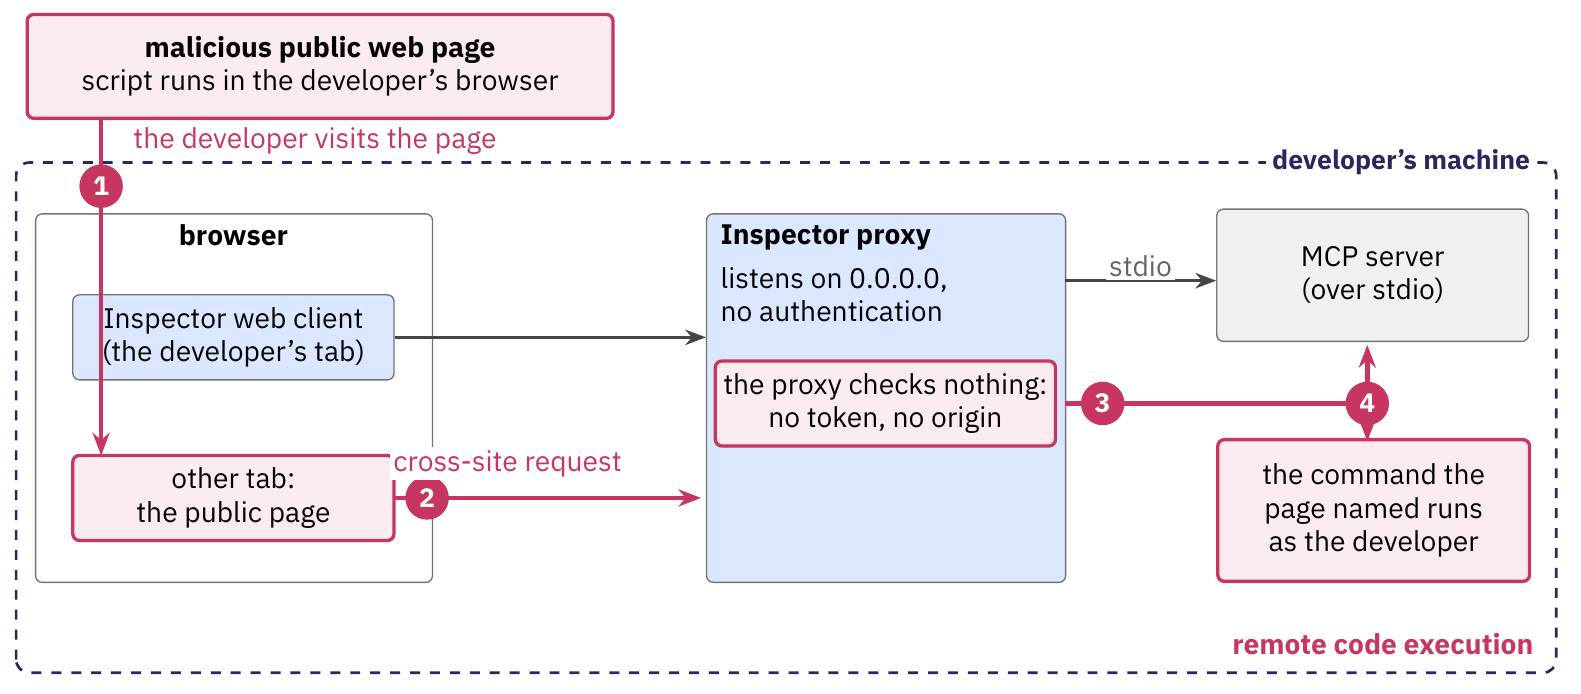
\includegraphics[width=\linewidth]{figures/inspector/inspector-exploit.png}
    \caption{Before version 0.14.1. A malicious page in the developer's browser sends a cross-site
    request to the proxy, which checks nothing and starts the command that the page names.}
    \label{fig:inspector-exploit}
  \end{subfigure}

  \medskip
  \begin{subfigure}{0.78\textwidth}
    \centering
    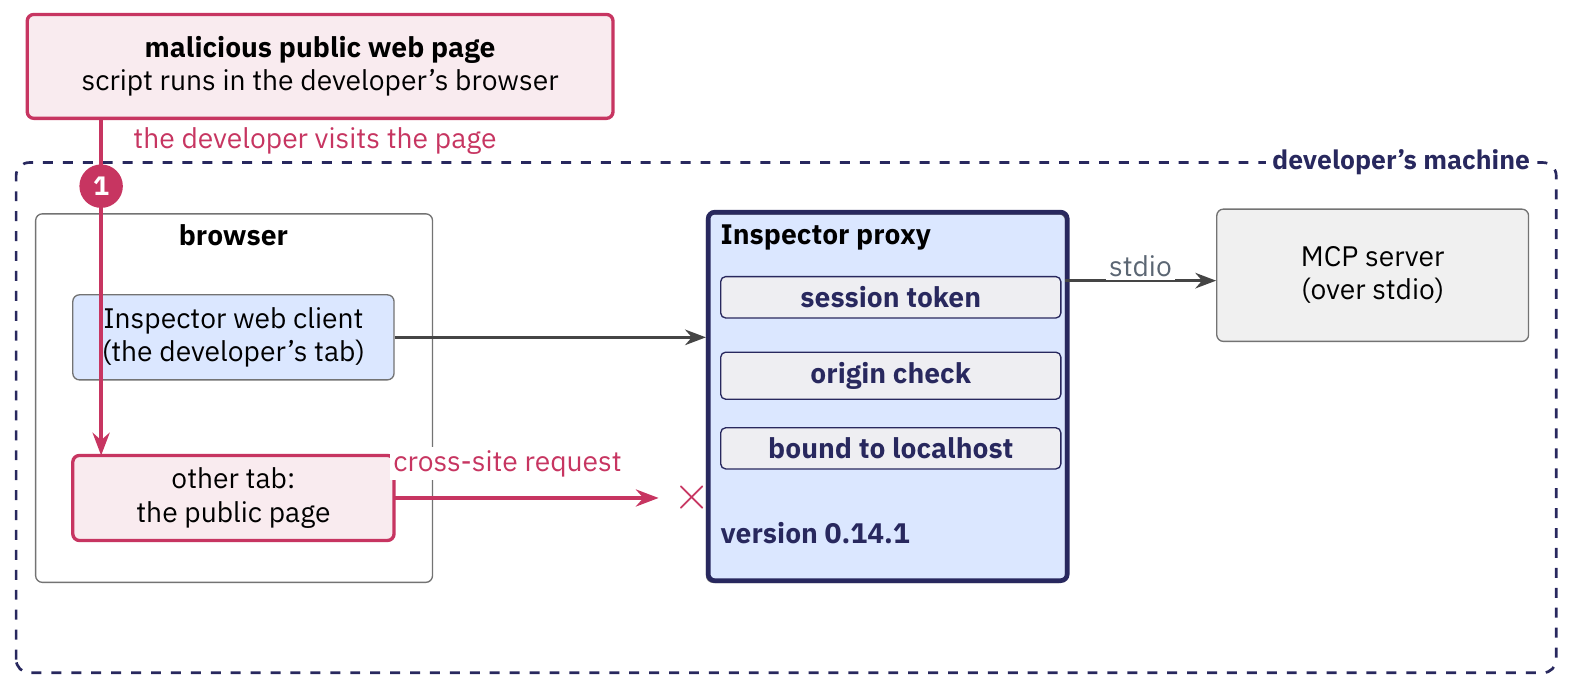
\includegraphics[width=\linewidth]{figures/inspector/inspector-fixed.png}
    \caption{From version 0.14.1. The proxy checks the session token and the origin of each
    request and refuses the same request, and the binding to localhost keeps other machines on the
    network out.}
    \label{fig:inspector-fixed}
  \end{subfigure}
  \caption{The Inspector vulnerability CVE-2025-49596 on the developer's machine, before and after
  the fix. Magenta marks the attack, from the adversary's page to the command it starts, and the
  numbered circles give the order of its steps.}
  \label{fig:inspector-replay}
\end{figure*}

The attack required nothing from the developer except a visit to a web page.
\Cref{fig:inspector-exploit} shows the developer's machine during the attack, with the browser's
two tabs on the left, the proxy in the middle and the MCP server on the right. The numbered circles
trace the attack from the malicious page to the command that it starts.

The attack began with the developer running the Inspector: the web client talked to the proxy, and
the proxy started the MCP server over stdio. In the vulnerable versions, the proxy listened on
0.0.0.0 and asked for no authentication. A program that listens on 0.0.0.0 accepts connections on
every network interface of the machine, so other machines on the same network can connect to it as
well.

A public page could reach the proxy through the developer's browser. A \textbf{cross-site request}
is a request that a page sends to a site other than its own. Browsers send such requests, because
pages routinely load images from other sites and submit forms to them.

The browser lets the sending page read the response only when the receiving server allows it. An
ordinary request, such as a GET request for an image, still arrives at the receiver and is
processed. The attack needed no response, because starting the command was its whole effect.

The page addressed its request to 0.0.0.0. The browser delivered it to the developer's own machine
because of the \textbf{0.0.0.0-day}, a browser flaw that let public web pages reach services on the
visitor's machine by sending requests to the address 0.0.0.0. This use of the address is separate
from the proxy's listening on 0.0.0.0, which exposed the proxy to other machines on the network.

A second route to the same proxy was \textbf{DNS rebinding}. In DNS rebinding, the attacker's domain
name first resolves to the attacker's server, which delivers the page, and then to a local address.
The browser still treats the page's later requests as requests to the page's own domain, so it lets
them through, and they reach a service on the visitor's machine.

Along the 0.0.0.0 route, the attack proceeded as follows, with its steps numbered as in
\cref{fig:inspector-exploit}:
\be
\item \textbf{The developer visits a malicious page.} The adversary controls a public web page, and
its script runs in the developer's browser, in a tab beside the Inspector.
\item \textbf{The page sends a cross-site request to the proxy.} The request names a command for
the proxy to start, and the 0.0.0.0 address carries it to the developer's own machine.
\item \textbf{The proxy accepts the request.} The proxy checks neither a token nor which page sent
the request, so it starts the named command as if it were an MCP server to be run over stdio.
\item \textbf{The command runs as the developer.} The command runs with the developer's rights. A
visit to one page has given the adversary remote code execution.
\ee

\subsection{The fix and the trust boundary}
\label{sec:inspector-fix}

Version 0.14.1 closed the vulnerability by making the proxy check who sends each request and by
limiting which machines can reach it \citep{mcp-inspector}. \Cref{fig:inspector-fixed} shows the
same request stopped at the proxy. The protections are the following:
\bi
\item \textbf{Session token.} The proxy requires its session token on every request to its API.
The token reaches the developer's own web client through a URL that carries it, which the
Inspector prints when it starts. A page from another site does not know the token, so its requests
are refused.
\item \textbf{Origin check.} An origin check examines the Origin header of a request, which
names the origin of the page that sent it, the scheme, host and port of its address
(\cref{sec:mcpcontract-http}). The proxy rejects a request whose Origin header names a page other
than the Inspector's web client.
The browser sets this header itself, and a script on the page cannot change it.
\item \textbf{Binding to localhost.} The proxy listens only on localhost, the address through which
a machine reaches its own services. Other machines on the network can no longer connect to it.
\ei

These protections close different routes. The session token stops the malicious page, because the
page does not know it, and the origin check rejects any request whose Origin header names another
site. Binding to localhost cannot stop the page, because the developer's browser runs on
the developer's own machine. The 0.0.0.0 route worked even against a service that listened only on
localhost \citep{lumelsky2025inspector}, and DNS rebinding sends the page's requests to a local
address by design.

Binding to localhost stops every other machine on the network. In the vulnerable versions, any such
machine could have sent the same request directly, with no browser involved.

The MCP specification asks for similar protections in a server that uses Streamable HTTP. Such a
server must validate the Origin header of every incoming connection to prevent DNS rebinding
(\cref{sec:mcpcontract}), should bind only to localhost when it runs locally, and should
authenticate all connections \citep{mcp-spec-2026}. The Inspector's proxy offers no tools of its
own. It accepts MCP messages from the web client over the same HTTP transports as a server, so it
can be attacked in the same way, from pages in the developer's browser.

A similar flaw was later found in another product. MCPJam, a third-party inspector for MCP servers,
listened on 0.0.0.0 by default, and a request to its server could make it start a command with no
check of the caller. The flaw was assigned CVE-2026-23744, with a CVSS 3.1 score of 9.8
\citep{nvd-cve-2026-23744}. Because the server listened on every interface, an attacker on the
network could reach it with a single HTTP request, without a browser.

Both flaws come from one missing check. A component that runs commands on request must check who
sends the request. The same rule applies to an MCP server, which must check every call it receives
even when the host has already checked it (\cref{sec:mcp}). When the check is missing, anyone who
can send the request can run code.

A \textbf{trust boundary} is the line between components that do not trust each other, at which
every request must be checked. Every trust boundary is a boundary in the sense of Lecture~4, an
interface that a request and its reply cross. A boundary is a trust boundary only when the
components on its two sides do not trust each other.

The Inspector's proxy sits on a trust boundary. On one side are the pages open in the developer's
browser, which may come from any site. On the other side are the developer's files and processes,
which any process that the proxy starts can reach with the developer's rights. The vulnerable versions
treated every request as if it came from the Inspector's own web client.

The debugging tool is therefore a host with a trust boundary of its own, and that boundary needs
the same checks as any other. The Inspector flaw also illustrates the difference between a class of
weakness, a reported vulnerability and an attacker's use of it (\cref{sec:threats}), and a missing
origin check recurs in the attacks on OpenClaw (\cref{sec:openclaw}).

\subsection*{Key points}
\bi
\item The MCP Inspector is a host with no model: its client sends the same \demoref{tools/list} and
\demoref{tools/call} requests as the client of any other host, and a person chooses each call.
\item A call that the tool refuses, or whose arguments fail the server's validation, comes back in
the Inspector as a result with \demoref{isError} true and the server's reason, which is the tool
execution error that a host passes to the model.
\item No deadline travels with an MCP request, so a client's timeout only ends its wait, and a tool
that ignores cancellation may finish its work after the client has given up, which leaves the
outcome of the call unknown.
\item Like every host, the Inspector receives only a tool's definition and its results, so it shows
a poisoned description without warning and cannot reveal a changed implementation.
\item Before version 0.14.1, the Inspector's proxy required no authentication, so a cross-site
request from a malicious page could make it run a command as the developer (CVE-2025-49596,
weakness class CWE-306).
\item The fix added a session token and an origin check, which stop requests from other sites'
pages, and bound the proxy to localhost in place of every network interface, which stops requests
from other machines.
\item A component that runs commands on request, including a debugging tool such as the Inspector,
sits on a trust boundary and must check who sends each request.
\ei
